% Copyright 2004 by Till Tantau <tantau@users.sourceforge.net>.
%
% In principle, this file can be redistributed and/or modified under
% the terms of the GNU Public License, version 2.
%
% However, this file is supposed to be a template to be modified
% for your own needs. For this reason, if you use this file as a
% template and not specifically distribute it as part of a another
% package/program, I grant the extra permission to freely copy and
% modify this file as you see fit and even to delete this copyright
% notice. 

\documentclass{beamer}

% There are many different themes available for Beamer. A comprehensive
% list with examples is given here:
% http://deic.uab.es/~iblanes/beamer_gallery/index_by_theme.html
% You can uncomment the themes below if you would like to use a different
% one:
%\usetheme{AnnArbor}
%\usetheme{Antibes}
%\usetheme{Bergen}
%\usetheme{Berkeley}
%\usetheme{Berlin}
%\usetheme{Boadilla}
%\usetheme{boxes}
%\usetheme{CambridgeUS}
%\usetheme{Copenhagen}
%\usetheme{Darmstadt}
%\usetheme{default}
%\usetheme{Frankfurt}
%\usetheme{Goettingen}
%\usetheme{Hannover}
%\usetheme{Ilmenau}
%\usetheme{JuanLesPins}
%\usetheme{Luebeck}
%\usetheme{Madrid}
%\usetheme{Malmoe}
%\usetheme{Marburg}
\usetheme[right,hideothersubsections]{Marburg}
%\usetheme{Montpellier}
%\usetheme{PaloAlto}
%\usetheme{Pittsburgh}
%\usetheme{Rochester}
%\usetheme{Singapore}
%\usetheme{Szeged}
%\usetheme{Warsaw}
\useinnertheme{circles}

\usepackage{comment}
\usepackage{hyperref}
\hypersetup{
    colorlinks=true,
    linkcolor=blue,
    filecolor=magenta,      
    urlcolor=cyan,
}

\title{Increasing profit from fees of cryptocurrencies}

% A subtitle is optional and this may be deleted
\subtitle{}
\author[]{Besart Dollma \and Noa Oved {\\\small Advisor: Itay Tsabary}}
% - Give the names in the same order as the appear in the paper.
% - Use the \inst{?} command only if the authors have different
%   affiliation.

\institute[] % (optional, but mostly needed)
{
  Technion - Israel Institute of Technology
}
% - Use the \inst command only if there are several affiliations.
% - Keep it simple, no one is interested in your street address.

\date{October, 2018}
% - Either use conference name or its abbreviation.
% - Not really informative to the audience, more for people (including
%   yourself) who are reading the slides online

\subject{}
% This is only inserted into the PDF information catalog. Can be left
% out. 

% If you have a file called "university-logo-filename.xxx", where xxx
% is a graphic format that can be processed by latex or pdflatex,
% resp., then you can add a logo as follows:

% \pgfdeclareimage[height=0.5cm]{university-logo}{university-logo-filename}
% \logo{\pgfuseimage{university-logo}}

% Delete this, if you do not want the table of contents to pop up at
% the beginning of each subsection:
\AtBeginSection[]
{
  \begin{frame}<beamer>{Outline}
    \tableofcontents[currentsection,currentsubsection]
  \end{frame}
}

% Let's get started
\begin{document}

\begin{frame}
  \titlepage
\end{frame}

\begin{frame}{Outline}
  \tableofcontents
  % You might wish to add the option [pausesections]
\end{frame}

% Section and subsections will appear in the presentation overview
% and table of contents.


%%======================================================================%%
%%%%%%%%%%%%%%%%%%%%%%%%%%%CRYPTOCURRENCIES%%%%%%%%%%%%%%%%%%%%%%%%%%%%%%%%
\section{Cryptocurrencies}
%%%%%%%%%%%%%%%%%%%%%%%%%%%%%%%%%%%%%%%%%%%%%%%%%%%%%%%%%%%%%%%%%%%%%%%%%%%
\subsection*{Cryptocurrencies}

\begin{frame}{Cryptocurrencies}{}
  \begin{itemize}
  \item {A cryptocurrency is digital asset designed to work as a medium 
  of exchange that uses strong cryptography to secure financial 
  transactions, control the creation of additional units, and verify 
  the transfer of assets.}
  \begin{figure}
      \centering
      \includegraphics{1.jpg}
      %\caption{Cryptocurrencies}
      \label{fig:my_label1}
  \end{figure}
  \item {We will focus on Bitcoin.}
  \end{itemize}
\end{frame}
%%%%%%%%%%%%%%%%%%%%%%%%%%%%%%%%%%%%%%%%%%%%%%%%%%%%%%%%%%%%%%%%%%%%%%%%%%%
\subsection*{Blockchain}

\begin{frame}{Blockchain} % Frame 1
  \begin{itemize}
  \item {The validity of each cryptocurrency's coins is provided by a 
  blockchain.}
  \item {Each block typically contains a hash pointer as a link to a 
  previous block, a timestamp and transaction data.}
  \begin{figure}
      \centering
      \includegraphics[height=3cm]{2.png}
      %\caption{Blockchain}
      \label{fig:my_label2}
  \end{figure}
  \end{itemize}
\end{frame}

\begin{frame}{Blockchain} % Frame 2
    \begin{itemize}
        \item {Resistant to data modification.}
        \item {On average, every 10 minutes a new block is added to
        the blockchain.}
        \item {Block size is 1 MB.}
    \end{itemize}
\end{frame}
%%%%%%%%%%%%%%%%%%%%%%%%%%%%%%%%%%%%%%%%%%%%%%%%%%%%%%%%%%%%%%%%%%%%%%%%%%%
\subsection*{Transactions}

\begin{frame}{Transactions}
    \begin{itemize}
        \item {When transferring cryptocurrency from one party to another, 
        a transaction is created and added to the Mempool (explained 
        later).}
        \item {Among other things, transactions contain:}
        \begin{table}[]
            \centering
            \begin{tabular}{c|c}
                \hline
                ID & 672e2c74d410d0a5b689925155098c9a39 \\ 
                \hline
                Fee & 0.00015820 BTC \\
                \hline
                Size & 224 bytes \\
                \hline
                Depends & [ ] \\
                \hline
            \end{tabular}
            %\caption{Transaction data}
            \label{tab:my_label3}
        \end{table}
    \end{itemize}
\end{frame}
%%%%%%%%%%%%%%%%%%%%%%%%%%%%%%%%%%%%%%%%%%%%%%%%%%%%%%%%%%%%%%%%%%%%%%%%%%%
\subsection*{MemPool}

\begin{frame}{MemPool}
    \begin{itemize}
        \item {Mempool (`Memory'+`Pool') is a 
        pool of memorized, held data.}
        \item {The data that is being stored on the Mempool are unconfirmed 
        transactions that are currently stuck on the network.}
        \item {We will denote the size of the mempool by $n$.}
        \item {$n \approx 16000$.}
    \end{itemize}
\end{frame}
%%%%%%%%%%%%%%%%%%%%%%%%%%%%%%%%%%%%%%%%%%%%%%%%%%%%%%%%%%%%%%%%%%%%%%%%%%%
\subsection*{Miners}

\begin{frame}{Miners}
    \begin{itemize}
        \item {In cryptocurrency networks, mining is a validation of 
        transactions.}
        \item {For this effort, successful miners obtain new cryptocurrency 
        as a reward.}
        \item {For each transcation the miner includes in a block, he 
        collects its fee.}
        \item { $\Rightarrow$ The miner's motivation is to maximize the sum of 
        the fees of the transactions that he includes in the block. This
        needs to be done under the size and dependency constraints.}
        \end{itemize}
    
\end{frame}


%%======================================================================%%
%%%%%%%%%%%%The knapsack and dependency knapsack problems%%%%%%%%%%%%%%%%%
\section{The knapsack and dependency knapsack problems}
%%%%%%%%%%%%%%%%%%%%%%%%%%%%%%%%%%%%%%%%%%%%%%%%%%%%%%%%%%%%%%%%%%%%%%%%%%%
\subsection*{The knapsack problem}

\begin{frame}{The knapsack problem}
    \begin{block}{Definition}
    We are given a knapsack (block) of size $W$ and $n$ transactions 
    $ \{a_1,a_2,...,a_n\}$. \\ 
    Each transaction $a_i$ has size $s_i > 0$ and fee $f_i \geq 0$. \\ 
    We are to find $ I \subseteq [n] $ such that: \\
    $$ I = \arg \max_{J \subseteq[n]} \{\sum_{j\in J} f_j\} $$ such that 
    $$ \sum_{j\in J} s_j \leq W $$
    \end{block}
\end{frame}
%%%%%%%%%%%%%%%%%%%%%%%%%%%%%%%%%%%%%%%%%%%%%%%%%%%%%%%%%%%%%%%%%%%%%%%%%%%
\subsection*{The dependency knapsack problem}

\begin{frame}{The dependency knapsack problem} % Frame 1
       \begin{block}{Definition}
    We are given a knapsack (block) of size $W$ and $n$ transactions 
    $ \{a_1,a_2,...,a_n\}$ as mentioned in the knapsack problem. \\ 
    Each transaction $a_i$ has in addition to its size and fee also a
    set of transaction which it depends upon. \\ 
    \end{block}
\end{frame}

\begin {frame}{The dependency knapsack problem} %Frame 2
    \begin{block}{Definition cont.}
    The goal is to find $\bar V \subseteq V$ such that: \\
    $$ \bar V = \arg \max_{J\subseteq V} \{\sum_{v\in J} f(v)\}$$ such 
    that \\
    $$ \sum_{v \in J} s(v) \leq W $$
    and the dependency constraints are preserved $\forall v \in \bar V$.
    \end{block}
\end{frame}

\begin{frame}{The dependency knapsack problem} % Frame 3
    \begin{itemize}
        \item  {No circular dependencies exist.}
        \item {We will treat the input as a directed acyclic graph (DAG)
        $ G = (V,E)$.}
        \item {Each node $v$ represents a transaction that has fee $f(v)$ 
        and size $s(v)$.}
        \item { Each edge $(i,j)$ represents that transaction $j$ is 
        dependent upon transaction $i$.}
        \item {Transaction $j$ can be selected iff transaction $m$ is 
        selected $\forall (m,j)\in E$.}
    \end{itemize}
\end{frame}

\begin {frame}{The dependency knapsack problem} %Frame 4
    \begin{example}
    \begin{itemize}
        \item {The knapsack size is $W=11$.}
        \begin{figure}
            \centering
            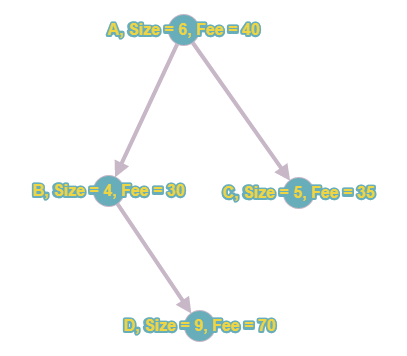
\includegraphics[height=4cm]{Figure1v2.png}
            \caption{Example of Knapsack with dependencies}
            %\label{fig:my_label}
        \end{figure}
        \item {Every transaction is dependent upon $A$, hence $A$ must be 
        selected.} \pause {Optimal solution is $\{A,C\}$.}
    \end{itemize}
    \end{example}
\end{frame}
%%%%%%%%%%%%%%%%%%%%%%%%%%%%%%%%%%%%%%%%%%%%%%%%%%%%%%%%%%%%%%%%%%%%%%%%%%%
\begin{frame}{NP-Completeness}
    \begin{itemize}
        \item {The decision problem form of the knapsack problem is 
        NP-complete.}
        \item {The dependency knapsack problem is a generalization of the 
        knapsack problem $\Rightarrow$ also NP-Complete.}
        \item {Thus there is no known algorithm both correct and polynomial
        for any of the problems.}
    \end{itemize}
\end{frame}

%%======================================================================%%
%%%%%%%%%%%%%%%%%%%%%%%%%%%%%Solutions%%%%%%%%%%%%%%%%%%%%%%%%%%%%%%%%%%%%%
\section {Solutions}
%%%%%%%%%%%%%%%%%%%%%%%%%%%%%%%%%%%%%%%%%%%%%%%%%%%%%%%%%%%%%%%%%%%%%%%%%%%
\subsection* {Knapsack solvers}
%%%%%%%%%%%%%%%%%%%%%%%%%%%%%%%%%%%%%%%%%%%%%%%%%%%%%%%%%%%%%%%%%%%%%%%%%%%
\subsubsection* {Exhaustive Search}

\begin{frame}{Knapsack solvers}{Exhaustive Search}
    \begin{itemize}
        \item {Trivial approach.}
        \item {Check all the subsets $J \subseteq [n]$.}
        \item{Optimal solution.}
        \item {Runtime is $ \mathcal{O}(2^n)$, hence exponential.}
        \item {We remind that $n \approx 16000$, therefore infeasible.}
    \end{itemize}
\end{frame}
%%%%%%%%%%%%%%%%%%%%%%%%%%%%%%%%%%%%%%%%%%%%%%%%%%%%%%%%%%%%%%%%%%%%%%%%%%%
\subsubsection*{Dynamic Programming}

\begin{frame}{Knapsack solvers}{Dynamic Programming}
    \begin{itemize}
        \item {Assume $s_1,s_2,...,s_n,W \in \mathbb N$. It holds on real 
        data.}
        \item {For each $ k\in \{0,1,...,n\}$ and for each 
        $w\in \{0,1,...,W\} $ define:}
          \item {$F(k,w) \triangleq$  the maximal profit when 
        choosing from transactions $\{a_1,...,a_k\}$ and the size of the 
        block is $w$.}
        \item { It holds:
            \begin{equation*}
                F(k,w) = \begin{cases}
                0 & \text{$k = 0$ or $ w = 0$}\\
                F(k-1,w) & \text{$w,k > 0$ and $s_k > w$} \\
                \xi & \text{$w,k > 0$ and $s_k \leq w$}
                \end{cases}
            \end{equation*}
            $$ \xi = \max\{F(k-1,w), f_k + F(k-1,w-s_k)\} $$
            }
        \item {Optimal solution.}
        \item {Runtime is $\mathcal{O}(nW)$, hence pseudo-polynomial.}
    \end{itemize}
\end{frame}
%%%%%%%%%%%%%%%%%%%%%%%%%%%%%%%%%%%%%%%%%%%%%%%%%%%%%%%%%%%%%%%%%%%%%%%%%%%
\subsubsection*{Greedy approximation}

\begin{frame}{Knapsack solvers}{Greedy approximation}
    \begin{itemize}
        \item {Sort the transactions by the $\frac{f_i}{s_i}$ ratio in 
        descending order.}
        \item {Iterate in this order and add transactions to the block until
         the next transaction can't be added.}
        \item {Not optimal but a 2-approx.}
        \item {Runtime is $\mathcal{O}(n\log{n})$.}
    \end{itemize}
\end{frame}
%%%%%%%%%%%%%%%%%%%%%%%%%%%%%%%%%%%%%%%%%%%%%%%%%%%%%%%%%%%%%%%%%%%%%%%%%%%
\subsubsection*{$(1+\varepsilon)$ approximation}

\begin{frame}{Knapsack solvers}{$(1+\varepsilon)$ approximation} %Frame 1
    \begin{itemize}
        \item {Let $0 \leq \varepsilon \leq 1$.}
        \item {Denote by $greedySol$ the value of the greedy approximation 
        and let $$ a = \varepsilon \cdot greedySol $$}
        \item {Denote $$ V_a = \{a_i \mid f_i < a\} $$  
        $$ V_a^C = \{a_i \mid f_i \geq a\} $$}
        \item {For each $J \subseteq V_a^C$ such that 
        $|J| \leq \frac{2}{\varepsilon}$:}
        \begin{itemize}
            \item {Run the greedy approximation on $V_a$ with block size 
            $W'=W-\sum_{j\in J} s_j$ and denote the solution by $I_j$.}
        \end{itemize}
        \item {Output $I_j \cup J$ with maximal profit.}
    \end{itemize}
\end{frame}

\begin{frame}{Knapsack solvers}{$(1+\varepsilon)$ approximation} %Frame 2
    \begin{itemize}
        \item {Not optimal but a $(1+\varepsilon)$ approx.}
        \item {Runtime is $\mathcal{O}(n^{1+\frac{2}{\varepsilon}}\cdot
        \log{n})$.}
        \item {If $\varepsilon \to 0$ we receive the exhaustive search. 
        Indeed it holds that $\frac{2}{\varepsilon} \to \infty$ 
        (non-polynomial).}
        \item {If $\varepsilon \to 1$ we receive the greedy approximation. 
        However the runtime is longer.}
    \end{itemize}
\end{frame}

%%%%%%%%%%%%%%%%%%%%%%%%%%%%%%%%%%%%%%%%%%%%%%%%%%%%%%%%%%%%%%%%%%%%%%%%%%%
%%%%%%%%%%%%%%%%%%%%%%%%%%%%%%%%%%%%%%%%%%%%%%%%%%%%%%%%%%%%%%%%%%%%%%%%%%%
\subsection* {Dependency knapsack solvers}

\begin{frame}{Solutions for the dependency knapsack problem} %Frame 1
    \begin{itemize}
        \item {We will discuss only the two approximations.}
        \item {The idea behind the algorithms remains the same.}
        \item {The algorithms are adjusted to supply the dependency 
        constraints.}
    \end{itemize}
    
\end{frame}

\begin{frame}{Solutions for the dependency knapsack problem} %Frame 2
        \begin{block}{Definition}
        For each transaction $v$ (node in the graph $G$)
        $$ Ancestor(v) \triangleq \{ j \mid \text{there exists a path from } 
        j \text{ to } v \text{ in } G \} $$
        \end{block}
        \begin{block}{Note}
        Pay attention that $v \in Ancestor(v)$.
        \end{block}
    
\end{frame}
%%%%%%%%%%%%%%%%%%%%%%%%%%%%%%%%%%%%%%%%%%%%%%%%%%%%%%%%%%%%%%%%%%%%%%%%%%%
\subsubsection* {Greedy approximation}

\begin{frame}{Dependency knapsack solvers}{Greedy approximation} %Frame 1
    \begin{block} {Algorithm}
        \begin{enumerate}
            \item {Calculate the sets $Ancestor(v) \text{ for all } v\in 
            V$.}
            \item {Pick $Ancestor(v)$ with the maximal
             $$\frac{\sum_{j\in Ancestor(v)} f(j)}{\sum_{j\in Ancestor(v)}
              s(j)} $$ ratio and add the transactions of the set to the
               knapsack. }
            \item {Remove the transactions we just added to the knapsack 
            from other sets and continue from 2 until we can't fit 
            anything in the block.}
        \end{enumerate}
    \end{block}
    \begin{itemize}
        \item {Runtime is $\mathcal{O} (n^3)$.}
    \end{itemize}
\end{frame}

\begin{frame}{Dependency knapsack solvers}{Greedy approximation} %Frame 2
    \begin{example}
    \begin{itemize}
        \item {The knapsack size is $W=11$.}
        \begin{figure}
            \centering
            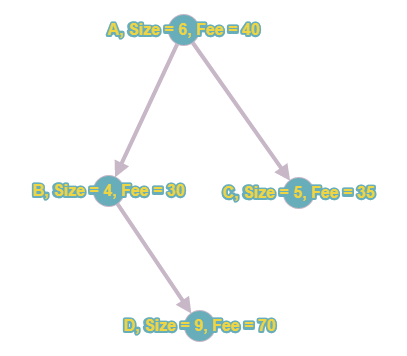
\includegraphics[height=4cm]{Figure1v2.png}
            \caption{Example of Knapsack with dependencies}
            %\label{fig:my_label}
        \end{figure}
        \item {We remind that the optimal solution is $\{A,C\}$.}
    \end{itemize}
    \end{example}
\end{frame}

\begin{frame}{Dependency knapsack solvers}{Greedy approximation} %Frame 3
    \begin{example}
         \begin{itemize}
            \item {$ Ancestor(D) = \{D,B,A\} \text{ and } 
            Ratio(D) = \frac{140}{19} \approx 7.36$.} \pause
            \item {$ Ancestor(B) = \{B,A\} \text{ and } 
            Ratio(B) = \frac{70}{10} = 7$.} \pause{}
            \item {$ Ancestor(C) = \{C,A\} \text{ and } 
            Ratio(C) = \frac{75}{11} \approx 6.81$.} \pause
            \item {$ Ancestor(A) = \{A\} \text{ and } 
            Ratio(A) = \frac{40}{6} \approx 6.66$.} \pause
            \item {The greedy approximation will eliminate $Ancestor(D)$
             because the size of the set 
             is 19 and the knapsack size is 11.} \pause {}
            \item {The algorithm will then add $Ancestor(B)$ to the 
            solution and remove $\{B,A\}$ from the other sets.} \pause
            \item {The algorithm will output $\{A,B\}$. Output value 
            is 70.} \pause 
            \item {Not optimal.}
        \end{itemize}
    \end{example}
\end{frame}

%%%%%%%%%%%%%%%%%%%%%%%%%%%%%%%%%%%%%%%%%%%%%%%%%%%%%%%%%%%%%%%%%%%%%%%%%%%
\subsubsection*{$(1+\varepsilon)$ approximation}

\begin{frame}{Dependency knapsack solvers}{$(1+\varepsilon)$ approximation}
% Frame 1
    \begin{itemize}
        \item {Similar to the $(1+\varepsilon)$ approximation for the 
        knapsack problem.}
        \item {Adjusted to the dependency knapsack problem using 
        $Ancestor(\cdot)$ sets.}
        \item {Runtime is $\mathcal{O}(n^{3+\frac{2}{\varepsilon}})$.}
    \end{itemize}
\end{frame}

\begin{frame}{Dependency knapsack solvers}{$(1+\varepsilon)$ approximation} 
% Frame 2
    \begin{example}
        \begin{itemize}
            \item {Let $\varepsilon = 0.1$}
            \item {$ a = \varepsilon \cdot greedySol = 7$}
            \item {$$V_a^C = \{a_i \mid f_i \geq a \} = \{A,B,C,D\}$$}
            \item {Therefore we will check all $J \subseteq V_a^C$ such 
            that $|J| \leq \frac{2}{\varepsilon} = 20$, in particular 
            $\{A,C\}$.}
            \item {In this example the algorithm outputs the optimal 
            solution.}
        \end{itemize}
    \end{example}
\end{frame}

%%%%%%%%%%%%%%%%%%%%%%%%%%%%%%%%%%%%%%%%%%%%%%%%%%%%%%%%%%%%%%%%%%%%%%%%%%%
%%%%%%%%%%%%%%%%%%%%%%%%%%%%Incremental%%%%%%%%%%%%%%%%%%%%%%%%%%%%%%%%%%%%
\subsection*{Incremental greedy approximation}

\begin{frame}{An incremental solution to the greedy approximation} %Frame 1
    \begin{itemize}
        \item {Suppose at time $t$ we have the solution of the dependency knapsack problem.}
        \item {Now suppose that at time $t+1$ some transactions were added to the
         mempool but no transactions were removed.}
        \item {Suppose also that the added transactions may be dependent on
         transactions from time $t$ but not vice verse.}
    \end{itemize}
     \begin{block}{}
        Can we solve the dependency knapsack at time $t+1$ using the
         solution at time $t$ and reduce the runtime?
        \end{block}
\end{frame}

\begin{frame}{An incremental solution to the greedy approximation} %Frame 2
         \begin{block}{Goal:}
         Improve the running time.
        \end{block}
    \begin{itemize}
        \item {$Ancestor(v)$ remains 
        identical for all the transactions which were also at time $t$.}
        \item {The solution value can't improve the solution value of the greedy approximation.}
        \item {In most cases we got the same solution value.}
    \end{itemize}
\end{frame}

\begin{frame}{An incremental solution to the greedy approximation} %Frame 3
    \begin{block}{Algorithm}
        \begin{enumerate}
            \item {Calculate $Ancestor(v)$ for all transactions $v$.}
            \item {Denote by $$ \alpha = \max_{v} \frac{\sum_{j\in Ancestor(v)}
             f(j)}{\sum_{j\in Ancestor(v)} s(j)} $$ the maximal ratio of fee 
             over size of the transactions that weren't in the previous 
             solution.}
            \item {Add to the solution all the $Ancestor(\cdot)$ sets from the 
            previous solution with a ratio bigger than $\alpha$ and 
            remove them from the mempool. Use the greedy approximation 
            algorithm on the transactions left on the mempool with the new size of 
            the block.}
        \end{enumerate}
    \end{block}
\end{frame}

%%======================================================================%%
%%%%%%%%%%%%%%%%%%%%%%%%%%%Implementation%%%%%%%%%%%%%%%%%%%%%%%%%%%%%%%%%%%
\section {Implementation}

\begin{frame}{Implementation}
    \begin{itemize}
        \item {We implemented the algorithms using 
        \href{https://www.python.org/}{Python}.}
        \item {Graphs aren't build in, hence we used the 
        \href{https://networkx.github.io/}{networkx} package.}
        \item {Everything can be found in our 
        \href{https://besartdollma.github.io/Increasing-profit-from-fees-of-cryptocurrencies/}{github}.}
        \item {Caching was disabled through out the tests.}
    \end{itemize}
\end{frame}
%%%%%%%%%%%%%%%%%%%%%%%%%%%%%%%%%%%%%%%%%%%%%%%%%%%%%%%%%%%%%%%%%%%%%%%%%%%%

%%======================================================================%%
%%%%%%%%%%%%%%%%%%%%%%%%%%%%%%%Results%%%%%%%%%%%%%%%%%%%%%%%%%%%%%%%%%%%%
\section{Results}
%%%%%%%%%%%%%%%%%%%%%%%%%%%%%%%%%%%%%%%%%%%%%%%%%%%%%%%%%%%%%%%%%%%%%%%%%%%%
\subsection*{The knapsack problem}
%%%%%%%%%%%%%%%%%%%%%%%%%%%%%%%%%%%%%%%%%%%%%%%%%%%%%%%%%%%%%%%%%%%%%%%%%%%%
\begin{frame}{The knapsack problem}{}  %Frame 2
    \begin{itemize}
        \item{Exhaustive search and dynamic programming are infeasible}
            \begin{enumerate}
                \item {For $n=20$ the exhaustive search runs on average 8 sec.}
                \item {Dynamic programming:}
                \begin{itemize}
                    \item {If $n=1000, W=1000$ runs on average 1 sec.}
                    \item {If $n =25, W = 1 $ MB (block size) runs on average 25 sec.}
                \end{itemize}
            \end{enumerate}
    \end{itemize}
\end{frame}

\begin{frame}{The knapsack problem}{}  %Frame 3
    \begin{itemize}
        \item{Picking the right $\varepsilon$ for the $(1+\varepsilon)$ approximation}
        \begin{enumerate}
            \item {Right $\varepsilon$ means a better solution of the $(1+\varepsilon)$ approximation than the greedy approximation.}
            \item {The right $\varepsilon$ is usually very small. This makes $\frac{2}{\varepsilon}$ very big $\Rightarrow$ long runtime (exponential on $\frac{2}{\varepsilon}$).}
            \item {Hence, if $|V_a^C| > 20$ we reduce it to 20 it by moving transactions to $V_a$.} 
            \item {$\Rightarrow$ The algorithm isn't a $(1+\varepsilon)$ approx.}
            \item {We studied different ways to pick which transactions to leave in $V_a^C$.}
        \end{enumerate}
    \end{itemize}
\end{frame}

\begin{comment}
%%EVERYTHING FROM HERE ON IS A COMMENT UNTIL YOU FIND \end{comment}
\begin{frame}{The knapsack problem}{Experiment I} %Frame 1
    \begin{itemize}
        \item {Let's compare the knapsack solvers head to head.}
    \end{itemize}
    \begin{block}{Experiment I}
     For each $1\leq n \leq 20$, we generated each time $n$ random 
     transactions $a_i$ such that $1\leq s_i,f_i\leq 100$. $W=1000$. The 
     data points are calculated as the average of 50 runs.
    \end{block}
\end{frame}

\begin{frame}{The knapsack problem}{Experiment I} %Frame 2
    \begin{figure}
        \centering
        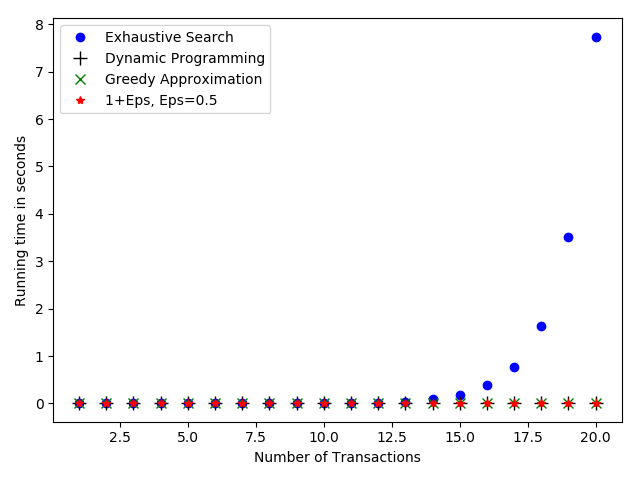
\includegraphics[height=6cm]{Figure2v2.png}
        \caption{Runtime in seconds as a function of $n$}
        %\label{fig:my_label}
    \end{figure}
\end{frame}

\begin{frame}{The knapsack problem}{Experiment I} %Frame 3
    \begin{figure}
        \centering
        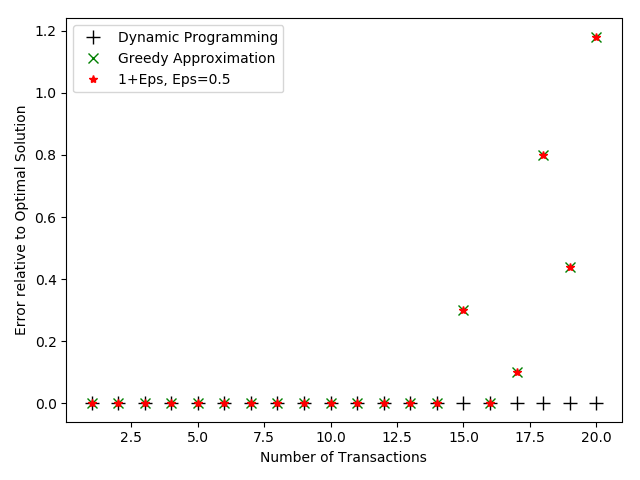
\includegraphics[height=6cm]{Figure3v2.png}
        \caption{Relative error as a function of $n$}
        %\label{fig:my_label}
    \end{figure}
\end{frame}
%%%%%%%%%%%%%%%%%%%%%%%%%%%%%%%%%%%%%%%%%%%%%%%%%%%%%%%%%%%%%%%%%%%%%%%%%%%%
\begin{frame}{The knapsack problem}{Experiment II} %Frame 4
    \begin{itemize}
        \item {Experiment I shows that exhaustive search is not feasible.}
        \item {Let's see how the other algorithms behave when the number of 
        transactions gets bigger.}
    \end{itemize}
    \begin{block}{Experiment II}
    The parameters are the same as in Experiment I, only this time 
    $n = 1,26,51,....,976$.
    \end{block}
\end{frame}

\begin{frame}{The knapsack problem}{Experiment II} %Frame 5
    \begin{figure}
        \centering
        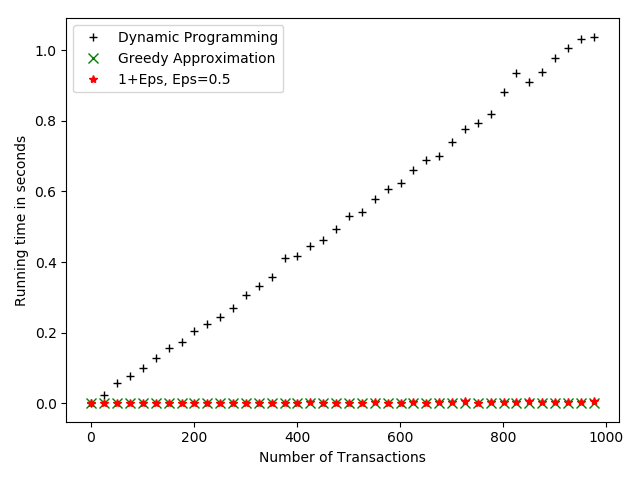
\includegraphics[height=6cm]{Figure4v2.png}
        \caption{Runtime in seconds as a function of $n$}
        %\label{fig:my_label}
    \end{figure}
\end{frame}

\begin{frame}{The knapsack problem}{Experiment II} %Frame 6
    \begin{figure}
        \centering
        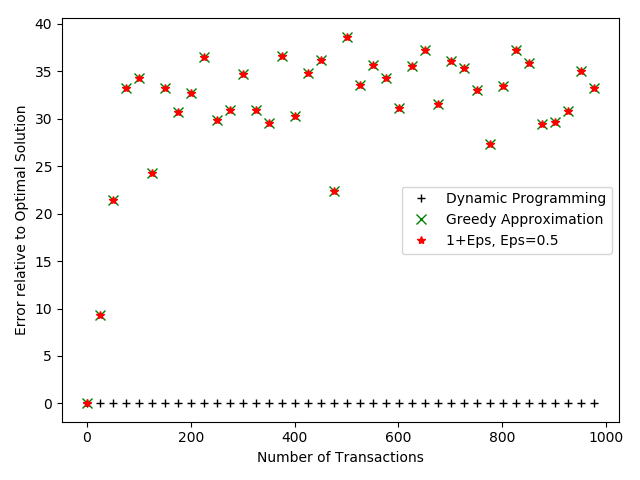
\includegraphics[height=6cm]{Figure5v2.png}
        \caption{Relative error as a function of $n$}
        %\label{fig:my_label}
    \end{figure}
\end{frame}
%%%%%%%%%%%%%%%%%%%%%%%%%%%%%%%%%%%%%%%%%%%%%%%%%%%%%%%%%%%%%%%%%%%%%%%%%%%%
\begin{frame}{The knapsack problem}{Experiment III} %Frame 7
    \begin{itemize}
        \item {From experiment II it looks like the dynamic programming 
        might handle a case of real data.}
        \item {It is optimal and it took around one second to solve an 
        instance of 1000 transactions.}
        \item {However let's alter the parameters a bit.}
    \end{itemize}
    \begin{block}{Experiment III}
    $$ W= 10^6 = 1 \text{ Mega} $$ 
    For each $1\leq n \leq 25$, we generated each time $n$ random transactions
    $a_i$ such that $1\leq s_i\leq 500$ and $1\leq f_i \leq 2000$. The 
    data points are calculated as the average of 25 runs.
    \end{block}
\end{frame}

\begin{frame}{The knapsack problem}{Experiment III} %Frame 8
    \begin{figure}
        \centering
        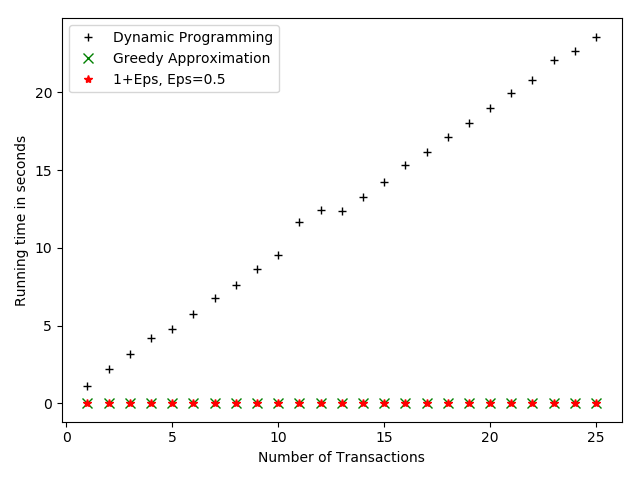
\includegraphics[height=6cm]{Figure6v2.png}
        \caption{Runtime in seconds as a function of $n$}
        %\label{fig:my_label}
    \end{figure}
\end{frame}
%%%%%%%%%%%%%%%%%%%%%%%%%%%%%%%%%%%%%%%%%%%%%%%%%%%%%%%%%%%%%%%%%%%%%%%%%%%%
\begin{frame}{The knapsack problem}{Experiment IV} %Frame 9
    \begin{itemize}
        \item {Experiment III shows that dynamic programming is also 
        infesiable.}
        \item {We are left with the two approximations.}
    \end{itemize}
    \begin{block}{Experiment IV}
    For each $n=1,21,41,...,981$ we generated each time $n$ random 
    transactions $a_i$ such that $1\leq s_i\leq 200$ and 
    $1\leq f_i \leq 100$. $W = 1000$. The data points are calculated as 
    the average of 50 runs.
    \end{block}
\end{frame}

\begin{frame}{The knapsack problem}{Experiment IV} %Frame 10
    \begin{figure}
        \centering
        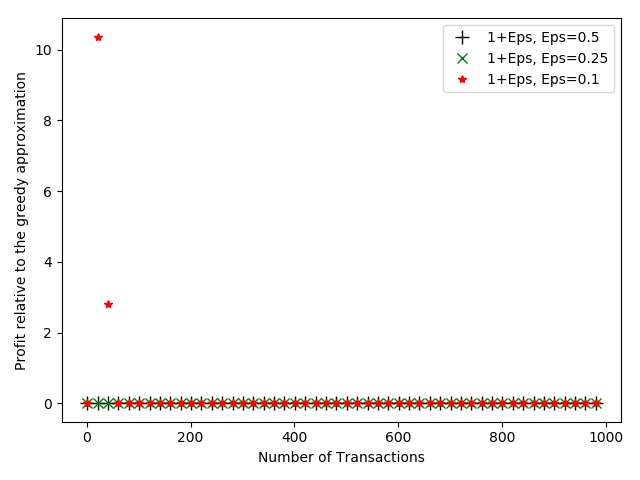
\includegraphics[height=6cm]{Figure7v2.png}
        \caption{Profit compared to greedy approximation as a function of 
        $n$}
        %\label{fig:my_label}
    \end{figure}
\end{frame}

\begin{frame}{The knapsack problem}{Experiment IV} %Frame 11
    \begin{figure}
        \centering
        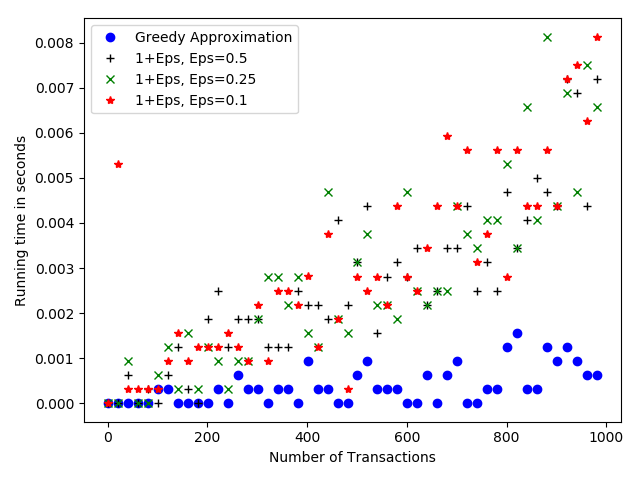
\includegraphics[height=6cm]{Figure8v2.png}
        \caption{Runtime in seconds as a function of $n$}
        %\label{fig:my_label}
    \end{figure}
\end{frame}
%%%%%%%%%%%%%%%%%%%%%%%%%%%%%%%%%%%%%%%%%%%%%%%%%%%%%%%%%%%%%%%%%%%%%%%%%%%%
\begin{frame}{The knapsack problem} %Frame 12
    \begin{itemize}
        \item {Experiment IV shows that picking the right $\varepsilon$ 
        might increase the profit.}
        \item {However the right $\varepsilon$ might be very small. This 
        means that $\frac{2}{\varepsilon}$ might be very big.}
        \item {We remind that the runtime of the $(1+\varepsilon)$ 
        approximation is exponential on $\frac{2}{\varepsilon}$.}
        \item {Hence $|V_a^C|$ shouldn't be too big, otherwise the algorithm
         won't be feasible.}
        \item {If $|V_a^C|>20$ we reduce it to 20 by moving the other 
        transactions to $V_a$. Now the algorithm isn't a $(1+\varepsilon)$ 
        approx.}
        \item {We studied the following reduce parameters:
            \begin{itemize}
                \item {Pick 20 random transactions.}
                \item {Pick the 20 transactions with the best $\frac{f_i}{s_i}$ 
                ratio.}
                \item{Pick the 20 transactions with the highest fee.}
                \item{Pick the 20 transactions with the biggest size.}
            \end{itemize}}
    \end{itemize}
\end{frame}
%%%%%%%%%%%%%%%%%%%%%%%%%%%%%%%%%%%%%%%%%%%%%%%%%%%%%%%%%%%%%%%%%%%%%%%%%%%%
\begin{frame}{The knapsack problem }{Experiment V} %Frame 13
    \begin{block}{Experiment V}
        For each $n=1,11,21,...,91$ we generated each time $n$ random 
        transactions $a_i$ such that $1\leq s_i\leq 200$ and 
        $1\leq f_i \leq 100$. $W=1000$. The data points are calculated as 
        the average of 5 runs.
    \end{block}
\end{frame}

\begin{frame}{The knapsack problem }{Experiment V} %Frame 14
    \begin{figure}
        \centering
        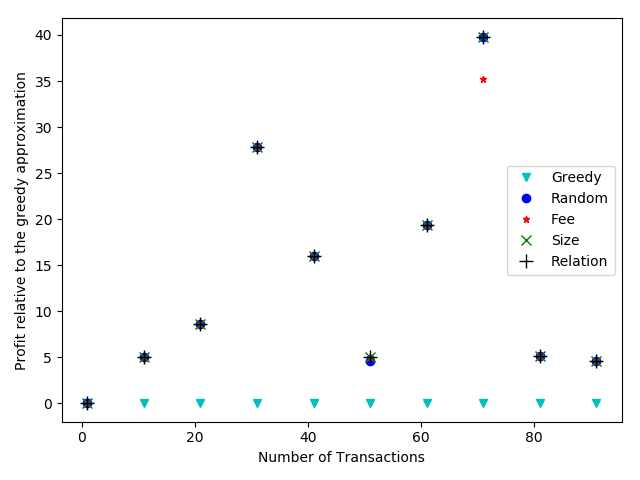
\includegraphics[height=6cm]{Figure9v2.png}
        \caption{Profit relative to the greedy approximation as a function 
        of $n$}
        %\label{fig:my_label}
    \end{figure}
\end{frame}
%%%%%%%%%%%%%%%%%%%%%%%%%%%%%%%%%%%%%%%%%%%%%%%%%%%%%%%%%%%%%%%%%%%%%%%%%%%%
\begin{frame}{The knapsack problem}{Experiment VI} %Frame 15
    \begin{itemize}
        \item {How does $\varepsilon$ influence the runtime and solution 
        value of the $(1+\varepsilon)$ approximation?}
    \end{itemize}
    \begin{block}{Experiment VI}
    We randomly generated 50 transactions such that $1\leq s_i,f_i \leq 200$.
    $W = 1000$. We decrease $\varepsilon$ using 
    $$ \varepsilon = \varepsilon\cdot 0.8 $$ until $\varepsilon \geq 0.01$.
    \end{block}
\end{frame}

\begin{frame}{The knapsack problem}{Experiment VI} %Frame 16
    \begin{figure}
        \centering
        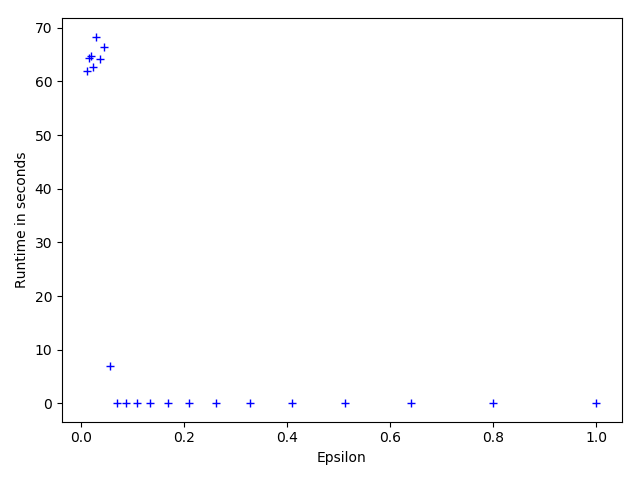
\includegraphics[height=6cm]{Figure10v2.png}
        \caption{Runtime in seconds as a function of $\varepsilon$}
        %\label{fig:my_label}
    \end{figure}
\end{frame}

\begin{frame}{The knapsack problem}{Experiment VI} %Frame 17
    \begin{figure}
        \centering
        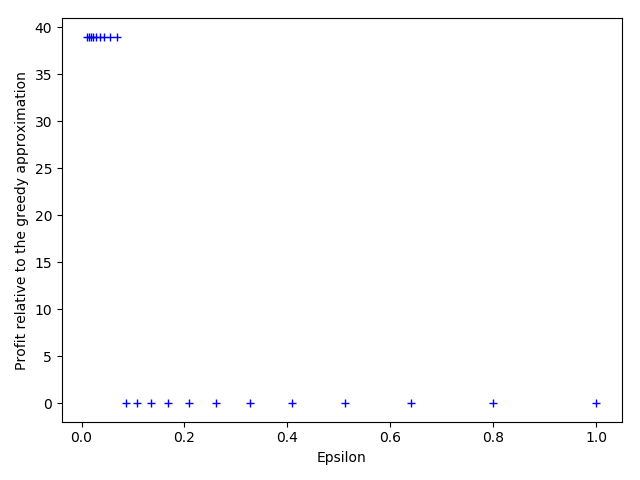
\includegraphics[height=6cm]{Figure11v2.png}
        \caption{Profit compared to greedy as a function of $\varepsilon$}
        %\label{fig:my_label}
    \end{figure}
\end{frame}
\end{comment}
%%%%%%%%%%%%%%%%%%%%%%%%%%%%%%%%%%%%%%%%%%%%%%%%%%%%%%%%%%%%%%%%%%%%%%%%%%%%
%%%%%%%%%%%%%%%%%%%%%%%%%%%%%%%%%%%%%%%%%%%%%%%%%%%%%%%%%%%%%%%%%%%%%%%%%%%%
\subsection* {The dependency knapsack problem}
%%%%%%%%%%%%%%%%%%%%%%%%%%%%%%%%%%%%%%%%%%%%%%%%%%%%%%%%%%%%%%%%%%%%%%%%%%%%
\begin{frame}{The dependency knapsack problem}{Experiment } %Frame 1
    \begin{itemize}
        \item {How do dependencies influence the runtime of the algorithms?}
        \item {The greedy approximation for the knapsack runs 
        $\mathcal{O}(n\cdot\log{n})$.}
        \item {The greedy approximation for the dependency knapsack runs 
        $\mathcal{O}(n^3)$.}
    \end{itemize}
    \begin{block}{Experiment }
    For each $n=1,11,21,...,141$ we generated each time $n$ random 
    transactions $a_i$ such that $1\leq s_i,f_i\leq 100$. $W=10000$. 
    The dependencies are also generated randomly such that there are no 
    circular dependencies. The result's data points are calculated as the average of 
    10 runs.
    \end{block}
\end{frame}

\begin{frame}{The dependency knapsack problem}{Experiment } %Frame 2
    \begin{figure}
        \centering
        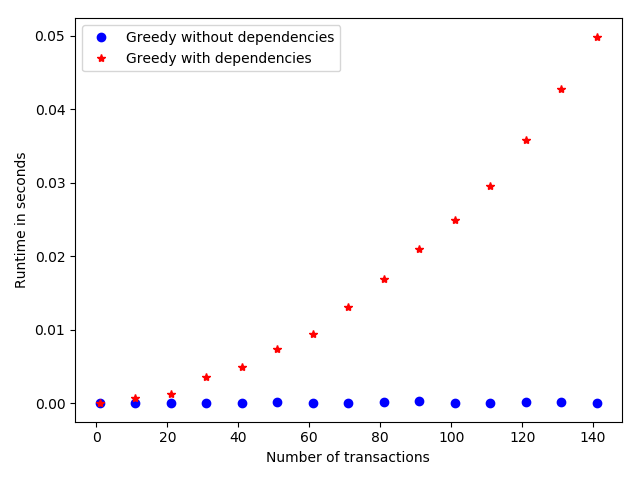
\includegraphics[height=6cm]{Figure12v2.png}
        \caption{Runtime in seconds as a function of $n$}
        %\label{fig:my_label}
    \end{figure}
\end{frame}
%%%%%%%%%%%%%%%%%%%%%%%%%%%%%%%%%%%%%%%%%%%%%%%%%%%%%%%%%%%%%%%%%%%%%%%%%%%%
\begin{comment}
\begin{frame}{The dependency knapsack problem}{Experiment II} %Frame 3
    \begin{itemize}
        \item {We want to compare between the two approximations.}
        \item {Also we want to explore the $(1+\varepsilon)$ approximation 
        for different $\varepsilon$.}    
    \end{itemize}
    \begin{block}{Experiment II}
    For each $n=1,11,21,...,141$ we generated each time $n$ random transactions
    $a_i$ such that $1\leq s_i \leq 200$ and $1\leq f_i\leq 100$. $W=10000$. 
    The dependencies are also generated randomly such that there are no 
    circular dependencies. The data points are calculated as the average of 
    10 runs. If $|V_a^C| > 15$ it is reduced to 15 using the fee criterion.
    \end{block}
\end{frame}

\begin{frame}{The dependency knapsack problem}{Experiment II} %Frame 4 
    \begin{figure}
        \centering
        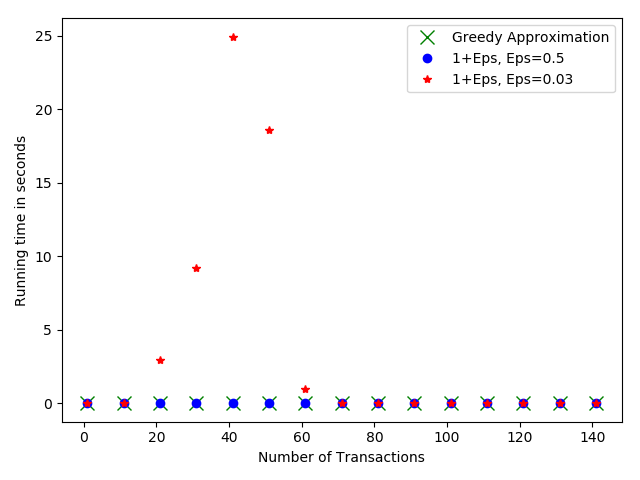
\includegraphics[height=6cm]{Figure13v2.png}
        \caption{Runtime in seconds as a function of $n$}
        %\label{fig:my_label}
    \end{figure}
\end{frame}

\begin{frame}{The dependency knapsack problem}{Experiment II} %Frame 5
    \begin{figure}
        \centering
        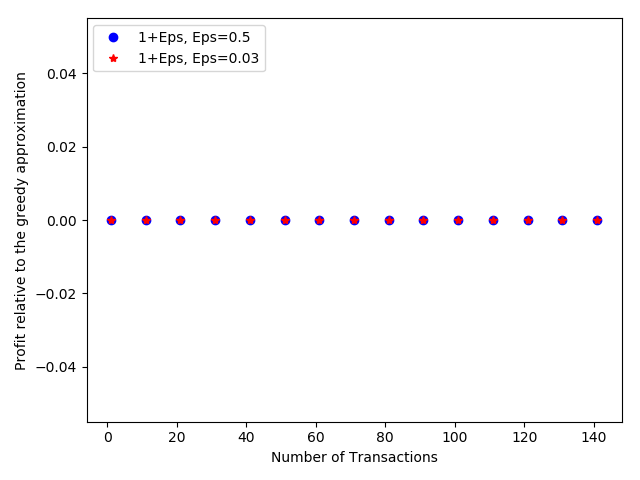
\includegraphics[height=6cm]{Figure14v2.png}
        \caption{Profit relative to the greedy approximation as a function
        of $n$}
        %\label{fig:my_label}
    \end{figure}
\end{frame}
\end{comment}
%%%%%%%%%%%%%%%%%%%%%%%%%%%%%%%%%%%%%%%%%%%%%%%%%%%%%%%%%%%%%%%%%%%%%%%%%%%%
%%%%%%%%%%%%%%%%%%%%%%%%%%%%%%%%%%%%%%%%%%%%%%%%%%%%%%%%%%%%%%%%%%%%%%%%%%%%
\subsection* {Real data}
%%%%%%%%%%%%%%%%%%%%%%%%%%%%%%%%%%%%%%%%%%%%%%%%%%%%%%%%%%%%%%%%%%%%%%%%%%%%
\begin{frame}{Real data}{} 
    \begin{itemize}
        \item {We checked the dependency knapsack approximations that we 
        implemented on real data.}
        \item {The data was sampled using the Bitcoin API.}
        \item {Every day, the first sample $t=1$ returns the whole mempool.}
        \item {Other samples $t>1$ through out the day return two sections:}
        \begin{itemize}
            \item {An added section that contains the transactions that are 
            added in the mempool after the last sample at $t-1$.}
            \item {The added transactions can be dependent upon transactions 
            that were in the mempool at time $t-1$ but not vice verse.}
            \item {A removed section that contains the transactions that are 
            removed from the mempool after the last sample at $t-1$.}
            \item {The removed section is usually empty.}
        \end{itemize}
    \end{itemize}
\end{frame}
%%%%%%%%%%%%%%%%%%%%%%%%%%%%%%%%%%%%%%%%%%%%%%%%%%%%%%%%%%%%%%%%%%%%%%%%%%%%
\begin{comment}
\begin{frame}{Real Data}{Experiment I}
    \begin{block}{Experiment I}
    First we explore how the approximations behave, especially how the 
    $(1+\varepsilon)$ approximation behaves for different $\varepsilon$. 
    In this experiment we tried $$\varepsilon \in 
    \{0.01,0.03,0.1,0.2,0.3,0.4,0.5,0.6,0.7,0.8,0.9,1\}$$   
    The data was collected on 28/08/2017 and the time sample is $t=1$.
    \end{block}
\end{frame}

\begin{frame}{Real Data}{Experiment I}
    \begin{figure}
        \centering
        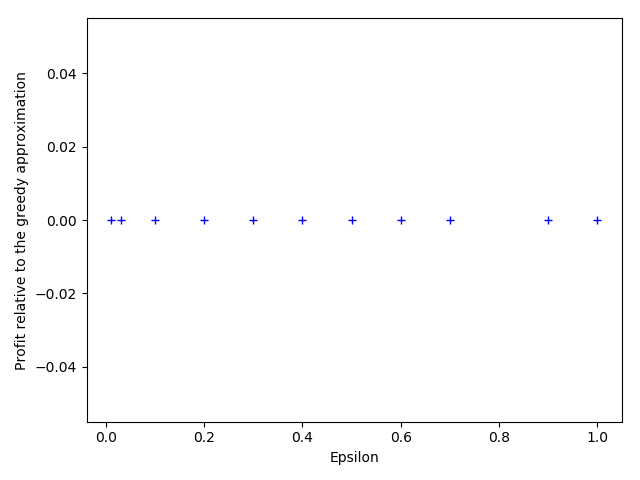
\includegraphics[height=6cm]{Figure15v2.png}
        \caption{Profit relative to the greedy approximation as a function 
        of $\varepsilon$}
        %\label{fig:my_label}
    \end{figure}
\end{frame}

\begin{frame}{Real Data}{Experiment I}
    \begin{figure}
        \centering
        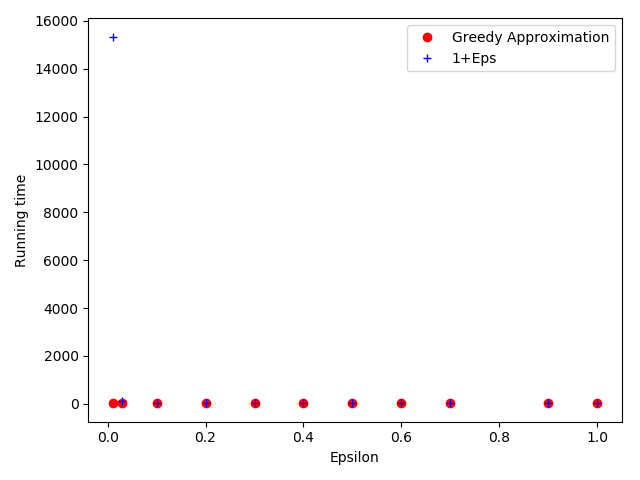
\includegraphics[height=6cm]{Figure16v2.png}
        \caption{Runtime in seconds as a function of $\varepsilon$}
        %\label{fig:my_label}
    \end{figure}
\end{frame}
\end{comment}
%%%%%%%%%%%%%%%%%%%%%%%%%%%%%%%%%%%%%%%%%%%%%%%%%%%%%%%%%%%%%%%%%%%%%%%%%%%%
\begin{frame}{Real Data}
    \begin{itemize}
        \item {For $\varepsilon > 0.03$ the two approximations yield the same solution almost every day because $V_a^C = \emptyset$.}
        \item {We explore the greedy approximation and $(1+\varepsilon)$ 
        approximation for $\varepsilon = 0.03$ through out 
        different days.}
        \item {The data was sampled at different days at time sample $t=1$.}
        \item {Furthermore, if $|V_a^C| > 10$ it is reduced to 10 using the
        fee criterion.}
    \end{itemize}
\end{frame}

\begin{frame}{Real Data}
    \begin{figure}
        \centering
        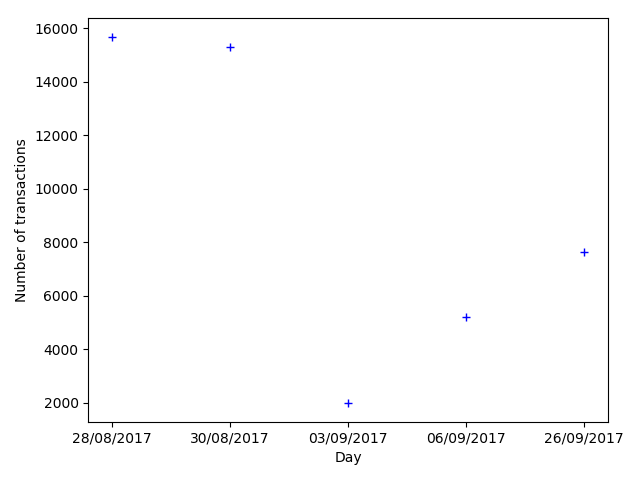
\includegraphics[height=6cm]{Figure17v2.png}
        \caption{$n$ at $t=1$ per day}
        %\label{fig:my_label}
    \end{figure}
\end{frame}


\begin{frame}{Real Data}
    \begin{figure}
        \centering
        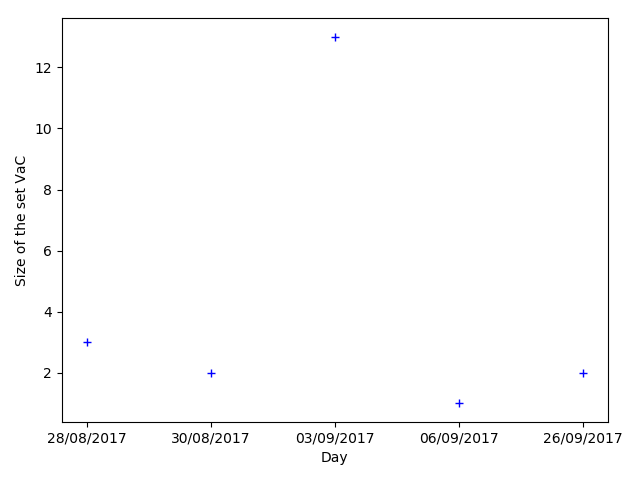
\includegraphics[height=6cm]{Figure20v2.png}
        \caption{$|V_a^C| $ per day when $\varepsilon=0.03$}
        %\label{fig:my_label}
    \end{figure}
\end{frame}

\begin{frame}{Real Data}
    \begin{figure}
        \centering
        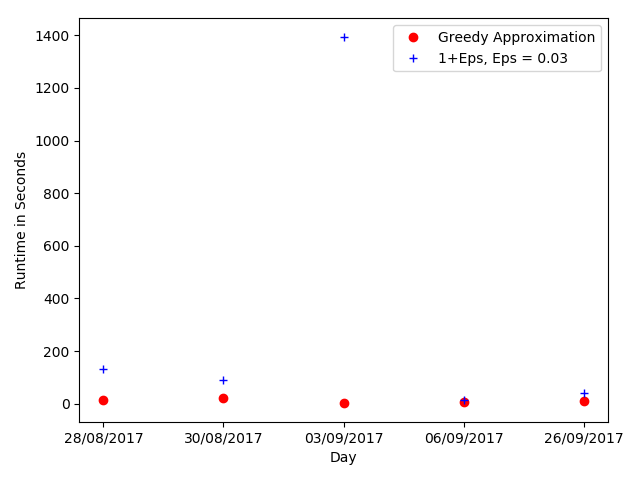
\includegraphics[height=6cm]{Figure21v2.png}
        \caption{Runtime in seconds per day}
        %\label{fig:my_label}
    \end{figure}
\end{frame}

\begin{frame}{Real Data}
    \begin{figure}
        \centering
        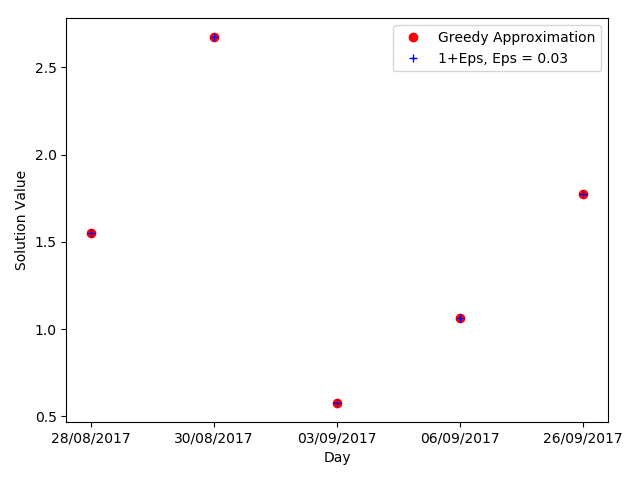
\includegraphics[height=6cm]{Figure22v2.png}
        \caption{The solution value per day}
        %\label{fig:my_label}
    \end{figure}
\end{frame}
%%%%%%%%%%%%%%%%%%%%%%%%%%%%%%%%%%%%%%%%%%%%%%%%%%%%%%%%%%%%%%%%%%%%%%%%%%%%
\begin{comment} %COMMENTED OUT
\begin{frame}{Real Data}{Experiment III}
    \begin{itemize}
        \item {We want to explore how the profit changes through out the 
        day.}
        \item {We mentioned that when we sample, the removed section is 
        usually empty.}
        \item {As such we expect the profit to increase.}
    \end{itemize}
    \begin{block}{Experiment III}
    We explore the profit as a function of $t$. The data was sampled on 
    28/08/2017.
    \end{block}
\end{frame}

\begin{frame}{Real Data}{Experiment III}
    \begin{figure}
        \centering
        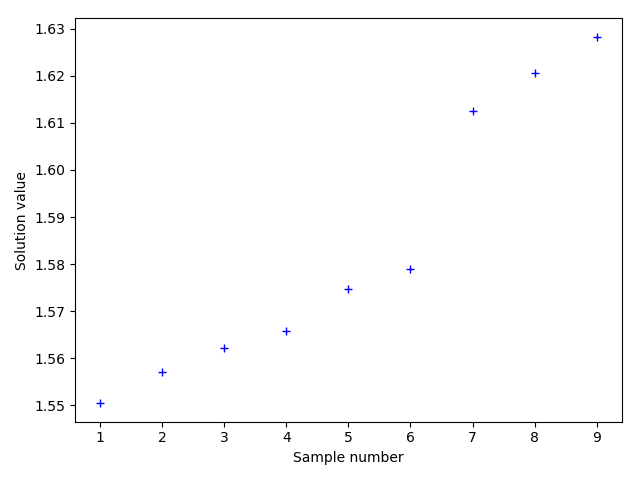
\includegraphics[height=6cm]{Figure23v2.png}
        \caption{Solution value as a function of $t$.}
        %\label{fig:my_label}
    \end{figure}
\end{frame}
\end{comment}
%%%%%%%%%%%%%%%%%%%%%%%%%%%%%%%%%%%%%%%%%%%%%%%%%%%%%%%%%%%%%%%%%%%%%%%%%%%%
%%%%%%%%%%%%%%%%%%%%%%%%%%%%%%%%%%%%%%%%%%%%%%%%%%%%%%%%%%%%%%%%%%%%%%%%%%%%
\subsection*{The incremental solution}
%%%%%%%%%%%%%%%%%%%%%%%%%%%%%%%%%%%%%%%%%%%%%%%%%%%%%%%%%%%%%%%%%%%%%%%%%%%%
\begin {comment}
\subsubsection*{Mock data}
%%%%%%%%%%%%%%%%%%%%%%%%%%%%%%%%%%%%%%%%%%%%%%%%%%%%%%%%%%%%%%%%%%%%%%%%%%%%
\begin{frame}{The incremental solution}{Mock Data - Experiment I}
    \begin{itemize}
        \item {We want to compare the two versions of the greedy 
        approximation.}
        \item {Incremental solution vs Non-Incremental solution.}
        \item {First we analyze them on mock data.}
    \end{itemize}
    \begin {block}{Experiment I}
    For each $1\leq n \leq 30$ we create a random instance of a dependency 
    knapsack problem with 100 transactions $a_i$ such that 
    $1\leq s_i,f_i \leq 100$ and $W=50000$. Then we add $n$ transactions to 
    this instance such that there are no circular dependencies. The data 
    points are the average of 25 runs.
    \end{block}
\end{frame}

\begin{frame}{The incremental solution}{Mock Data - Experiment I}
    \begin{figure}
        \centering
        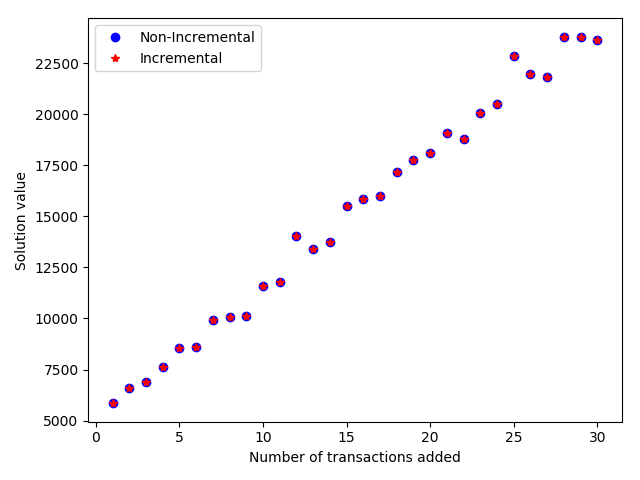
\includegraphics[height=6cm]{Figure24v2.png}
        \caption{Solution value as a function of the number of 
        transactions added}
        %\label{fig:my_label}
    \end{figure}
\end{frame}

\begin{frame}{The incremental solution}{Mock Data - Experiment I}
    \begin{figure}
        \centering
        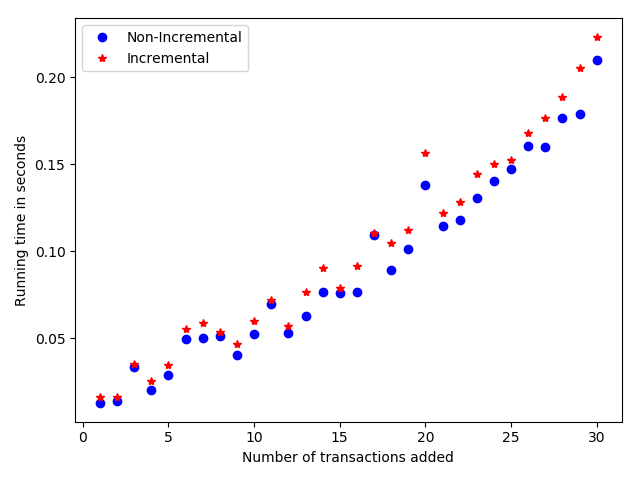
\includegraphics[height=6cm]{Figure25v2.png}
        \caption{Running time in seconds as a function of the number of 
        transactions added}
        %\label{fig:my_label}
    \end{figure}
\end{frame}
%%%%%%%%%%%%%%%%%%%%%%%%%%%%%%%%%%%%%%%%%%%%%%%%%%%%%%%%%%%%%%%%%%%%%%%%%%%%
\begin{frame}{The incremental solution}{Mock data - Experiment II}
    \begin{block}{Experiment II}
    We run the same experiment, only that now $n=1,11,21,...,291$.
    \end{block} 
\end{frame}

\begin{frame}{The incremental solution}{Mock Data - Experiment II}
    \begin{figure}
        \centering
        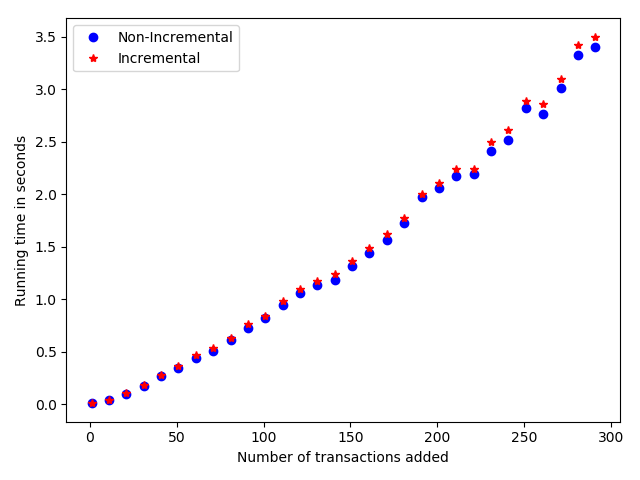
\includegraphics[height=6cm]{Figure26v2.png}
        \caption{Running time in seconds as a function of the number of 
        transactions added}
        %\label{fig:my_label}
    \end{figure}
\end{frame}
\end{comment}
%%%%%%%%%%%%%%%%%%%%%%%%%%%%%%%%%%%%%%%%%%%%%%%%%%%%%%%%%%%%%%%%%%%%%%%%%%%%
\subsubsection* {Real Data}
\begin{frame}{The incremental solution}{Real Data}
    \begin{itemize}
        %\item {We saw in mock data that the incremental solution doesn't 
        %improve the running time of the non-incremental solution.}
        %\item {This is because in our experiments only a small part of the 
        %previous solution became part of the new solution.}
        %\item {We want to run the incremental solution on real data.}
        \item {The real data provides the constraints needed in order to use 
        the incremental solution, since most of the time there are no 
        removed transactions but only added ones.}
    \end{itemize}
    \begin{block}{Experiment}
    This data was sampled on 28/08/2017. 
    \end{block}
\end{frame}

\begin{frame}{The incremental solution}{Real Data}
    \begin{figure}
        \centering
        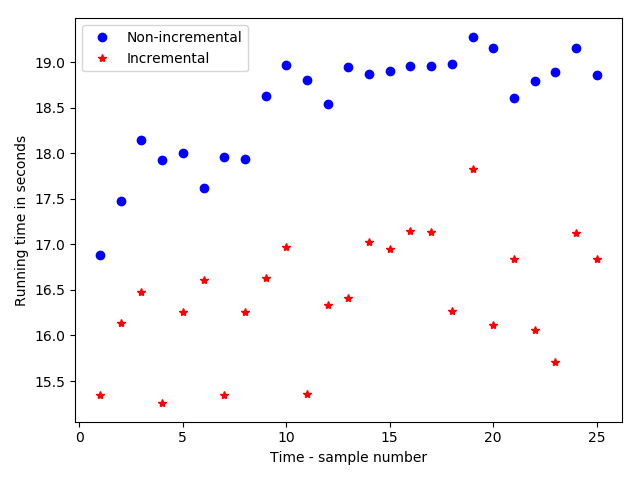
\includegraphics[height=6cm]{Figure27v2.png}
        \caption{Runtime in seconds as a function of $t$}
        %\label{fig:my_label}
    \end{figure}
\end{frame}

\begin{frame}{The incremental solution}{Real Data}
    \begin{figure}
        \centering
        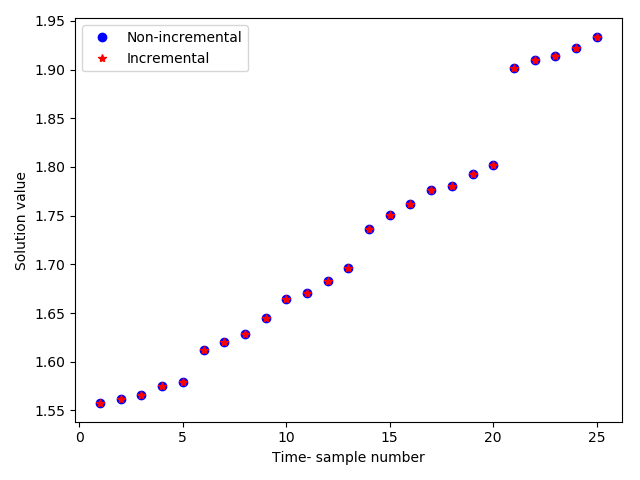
\includegraphics[height=6cm]{Figure28v2.png}
        \caption{Solution value as a function of $t$}
        %\label{fig:my_label}
    \end{figure}
\end{frame}
%%%%%%%%%%%%%%%%%%%%%%%%%%%%%%%%%%%%%%%%%%%%%%%%%%%%%%%%%%%%%%%%%%%%%%%%%%%%
\begin{comment}
\begin{frame}{The incremental solution}{Real Data - Experiment IV}
    \begin{itemize}
        \item {We saw that on real data the incremental solution makes a 
        difference.}
        \item {We get the same solution and save some time.}
    \end{itemize}
    \begin{block}{Experiment IV}
    Just to make sure we ran the same experiment on the data that was 
    collected on 03/09/2017. 
    \end{block}
\end{frame}

\begin{frame}{The incremental solution}{Real Data - Experiment IV}
    \begin{figure}
        \centering
        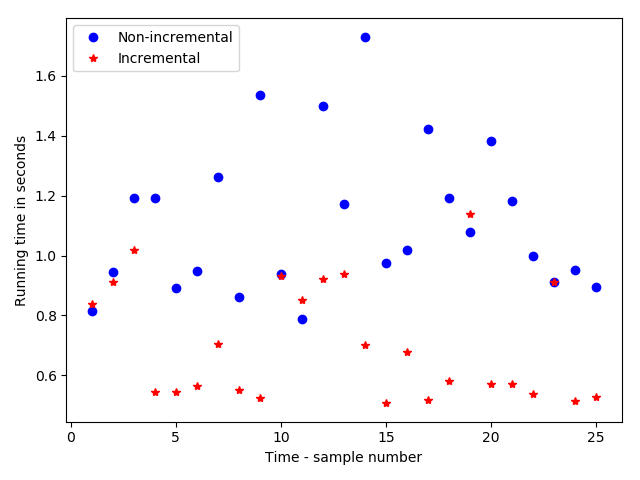
\includegraphics[height=6cm]{Figure29v2.png}
        \caption{Runtime in seconds as a function of $t$}
        %\label{fig:my_label}
    \end{figure}
\end{frame}

\begin{frame}{The incremental solution}{Real Data - Experiment IV}
    \begin{figure}
        \centering
        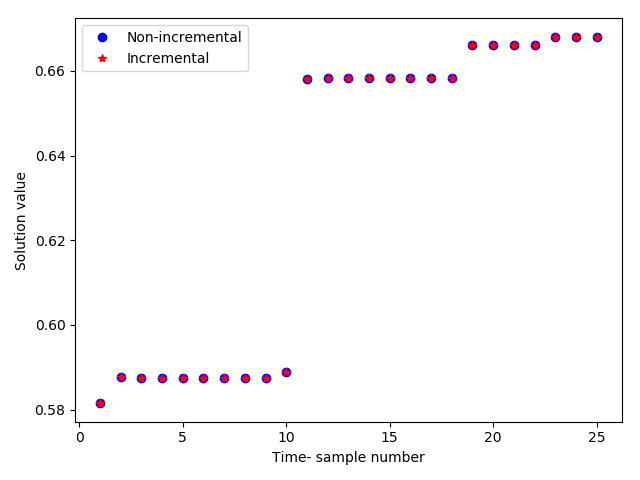
\includegraphics[height=6cm]{Figure30v2.png}
        \caption{Solution value as a function of $t$}
        %\label{fig:my_label}
    \end{figure}
\end{frame}
\end{comment}
%%%%%%%%%%%%%%%%%%%%%%%%%%%%%%%%%%%%%%%%%%%%%%%%%%%%%%%%%%%%%%%%%%%%%%%%%%%%
%==========================================================================%
%%%%%%%%%%%%%%%%%%%%%%%%%%%%%Conclusions%%%%%%%%%%%%%%%%%%%%%%%%%%%%%%%%%%%%
\section {Conclusions}
\begin{frame}{Conclusions} %Frame 1 
    \begin{itemize}
        \item {The exhaustive search algorithm and the dynamic programming algorithms are not feasible for big $n$ and big $W$.}
        \item {The dependency knapsack problem is harder to solve than the knapsack problem as we saw.}
    \end{itemize}
\end{frame}

\begin{frame}{Conclusions} %Frame 2 
    \begin{itemize}
        \item {The $(1+\varepsilon)$ approximation is not feasible for the dependency knapsack problem.} \item {Reason: the greedy approximation value $\gg$ fees of transactions $\Rightarrow \varepsilon \ll 1$ which means that $\frac{2}{\varepsilon}$ is big}
        \item { $\Rightarrow$ The algorithm becomes infesiable in terms of time and memory.}
        \item {On real data, the incremental solution algorithm gives the same results as the greedy approximation algorithm but it is faster most of the time.}
    \end{itemize}
\end{frame}

\end{document}

